\documentclass[aspectratio=169,11pt]{beamer}

\usepackage[utf8]{inputenc}
\usepackage[T1]{fontenc}
\usepackage[spanish,es-nodecimaldot]{babel}
\usefonttheme{serif}
\usepackage{booktabs}
\usepackage{tabularx}
\usepackage{array}
\usepackage{ragged2e}
\usepackage{amsmath,amssymb}
\usepackage{graphicx}
\usepackage{tikz}
\usepackage{listings}
\usepackage{xcolor}
\usepackage{pifont}
\usepackage{multicol}

\definecolor{uaoblue}{RGB}{31,58,95}
\definecolor{softgray}{RGB}{245,247,250}
\definecolor{textgray}{RGB}{70,70,70}
\definecolor{codebg}{RGB}{245,245,245}

\setbeamertemplate{navigation symbols}{}
\setbeamertemplate{items}[circle]
\setbeamertemplate{headline}{%
  \begin{beamercolorbox}[wd=\paperwidth,ht=2.6ex,dp=1.2ex,leftskip=0.4cm,rightskip=0.4cm]{section in head/foot}%
    \color{uaoblue}\scriptsize\textbf{UAO -- Incorporar Elementos de IA · Bloque Vision}
  \end{beamercolorbox}%
}
\setbeamertemplate{footline}{%
  \leavevmode%
  \hbox{%
    \begin{beamercolorbox}[wd=.78\paperwidth,ht=2.8ex,dp=1.2ex,leftskip=0.4cm]{author in head/foot}%
      \scriptsize Belalcazar · Gruezo -- Abril 2026
    \end{beamercolorbox}%
    \begin{beamercolorbox}[wd=.22\paperwidth,ht=2.8ex,dp=1.2ex,rightskip=0.4cm plus1fil]{date in head/foot}%
      \scriptsize\insertframenumber/\inserttotalframenumber
    \end{beamercolorbox}%
  }
}

\setbeamercolor{title}{fg=uaoblue}
\setbeamercolor{frametitle}{fg=uaoblue}
\setbeamercolor{structure}{fg=uaoblue}
\setbeamercolor{normal text}{fg=black,bg=white}
\setbeamercolor{block title}{fg=white,bg=uaoblue}
\setbeamercolor{block body}{bg=softgray}
\setbeamerfont{title}{series=\bfseries,size=\LARGE}
\setbeamerfont{subtitle}{size=\large}
\setbeamerfont{frametitle}{series=\bfseries,size=\large}

\lstset{
  basicstyle=\ttfamily\small,
  backgroundcolor=\color{codebg},
  frame=single,
  framerule=0pt,
  breaklines=true,
  columns=fullflexible,
  keepspaces=true,
  showstringspaces=false
}

\newcolumntype{Y}{>{\RaggedRight\arraybackslash}X}
\newcommand{\cmark}{\ding{51}}
\newcommand{\xmark}{\ding{55}}

\title{Clasificacion Medica Multimodal con \textbf{Mixture of Experts}}
\subtitle{Ablation Study del Router}
\author{Sebastian Belalcazar Mosquera \and Manuel Alejandro Gruezo\\Docente: Carlos Andres Ferro Sanchez}
\institute{Universidad Autonoma de Occidente}
\date{Abril 2026}

\begin{document}

% Portada
\begin{frame}[plain]
  \vspace{0.7cm}
  {\color{uaoblue}\LARGE\bfseries Clasificacion Medica Multimodal con \textbf{Mixture of Experts} \par}
  \vspace{0.3cm}
  {\color{uaoblue}\large Ablation Study del Router \par}
  \vspace{0.8cm}
  {\normalsize \textbf{Sebastian Belalcazar Mosquera} \quad -- \quad \textbf{Manuel Alejandro Gruezo} \par}
  \vspace{0.2cm}
  {\normalsize Docente: Carlos Andres Ferro Sanchez \par}
  \vspace{0.2cm}
  {\normalsize Universidad Autonoma de Occidente -- Abril 2026 \par}
  \vfill
\end{frame}

\begin{frame}{1. El problema y la pregunta cientifica}
\begin{itemize}
  \item Los sistemas clinicos reales procesan \textbf{multiples modalidades} (rayos X, dermoscopia, CT) sin saber de antemano que reciben.
  \item Un modelo por modalidad no escala; un modelo generalista pierde especializacion.
  \item \textbf{MoE} resuelve el dilema: un \emph{router} activa dinamicamente al experto adecuado.
\end{itemize}

\vspace{0.35cm}
\begin{block}{Pregunta cientifica central}
\centering
\large\textbf{\textquestiondown Justifica el Vision Transformer su costo computacional como router frente a metodos estadisticos clasicos operando sobre los mismos embeddings?}
\end{block}
\end{frame}

\begin{frame}{2. Datasets -- 5 modalidades, sin metadatos}
\small
\begin{tabularx}{\textwidth}{c Y Y c c}
\toprule
\# & Dataset & Modalidad & Clases & Volumen \\
\midrule
1 & NIH ChestX-ray14 & Rayos X 2D & 5 patol. & \textasciitilde112 K img \\
2 & ISIC 2019 & Dermoscopia 2D & 9 & \textasciitilde25 K img \\
3 & Osteoarthritis & RX rodilla 2D & 3 & \textasciitilde10 K img \\
4 & LUNA16 & CT pulmonar 3D & 2 & 888 vol. \\
5 & Pancreatic Cancer & CT abdominal 3D & 2 & \textasciitilde281 vol. \\
\bottomrule
\end{tabularx}

\vspace{0.35cm}
\begin{block}{Restriccion}
El sistema recibe \textbf{solo la imagen}: nada de texto, ni modalidad, ni nombre de archivo. Las soluciones que pasen metadatos pierden 20\%.
\end{block}
\end{frame}

\begin{frame}[fragile]{3. Preprocesador adaptativo -- sin metadatos}
\begin{lstlisting}
rank(x) == 4  ->  imagen 2D  ->  Resize 224x224 + normalizacion ImageNet
rank(x) == 5  ->  volumen 3D ->  Resize 64x64x64 + HU [-1000, 400]
\end{lstlisting}

\begin{itemize}
  \item Sin \texttt{if modality == "xray"}: la modalidad \textbf{se infiere}, no se recibe.
  \item Elimina por diseno la penalizacion de -20\% por uso de metadatos.
  \item Permite que una misma interfaz sirva para PNG/JPEG/NIfTI.
\end{itemize}
\end{frame}

\begin{frame}{4. Arquitectura del sistema MoE}
\centering
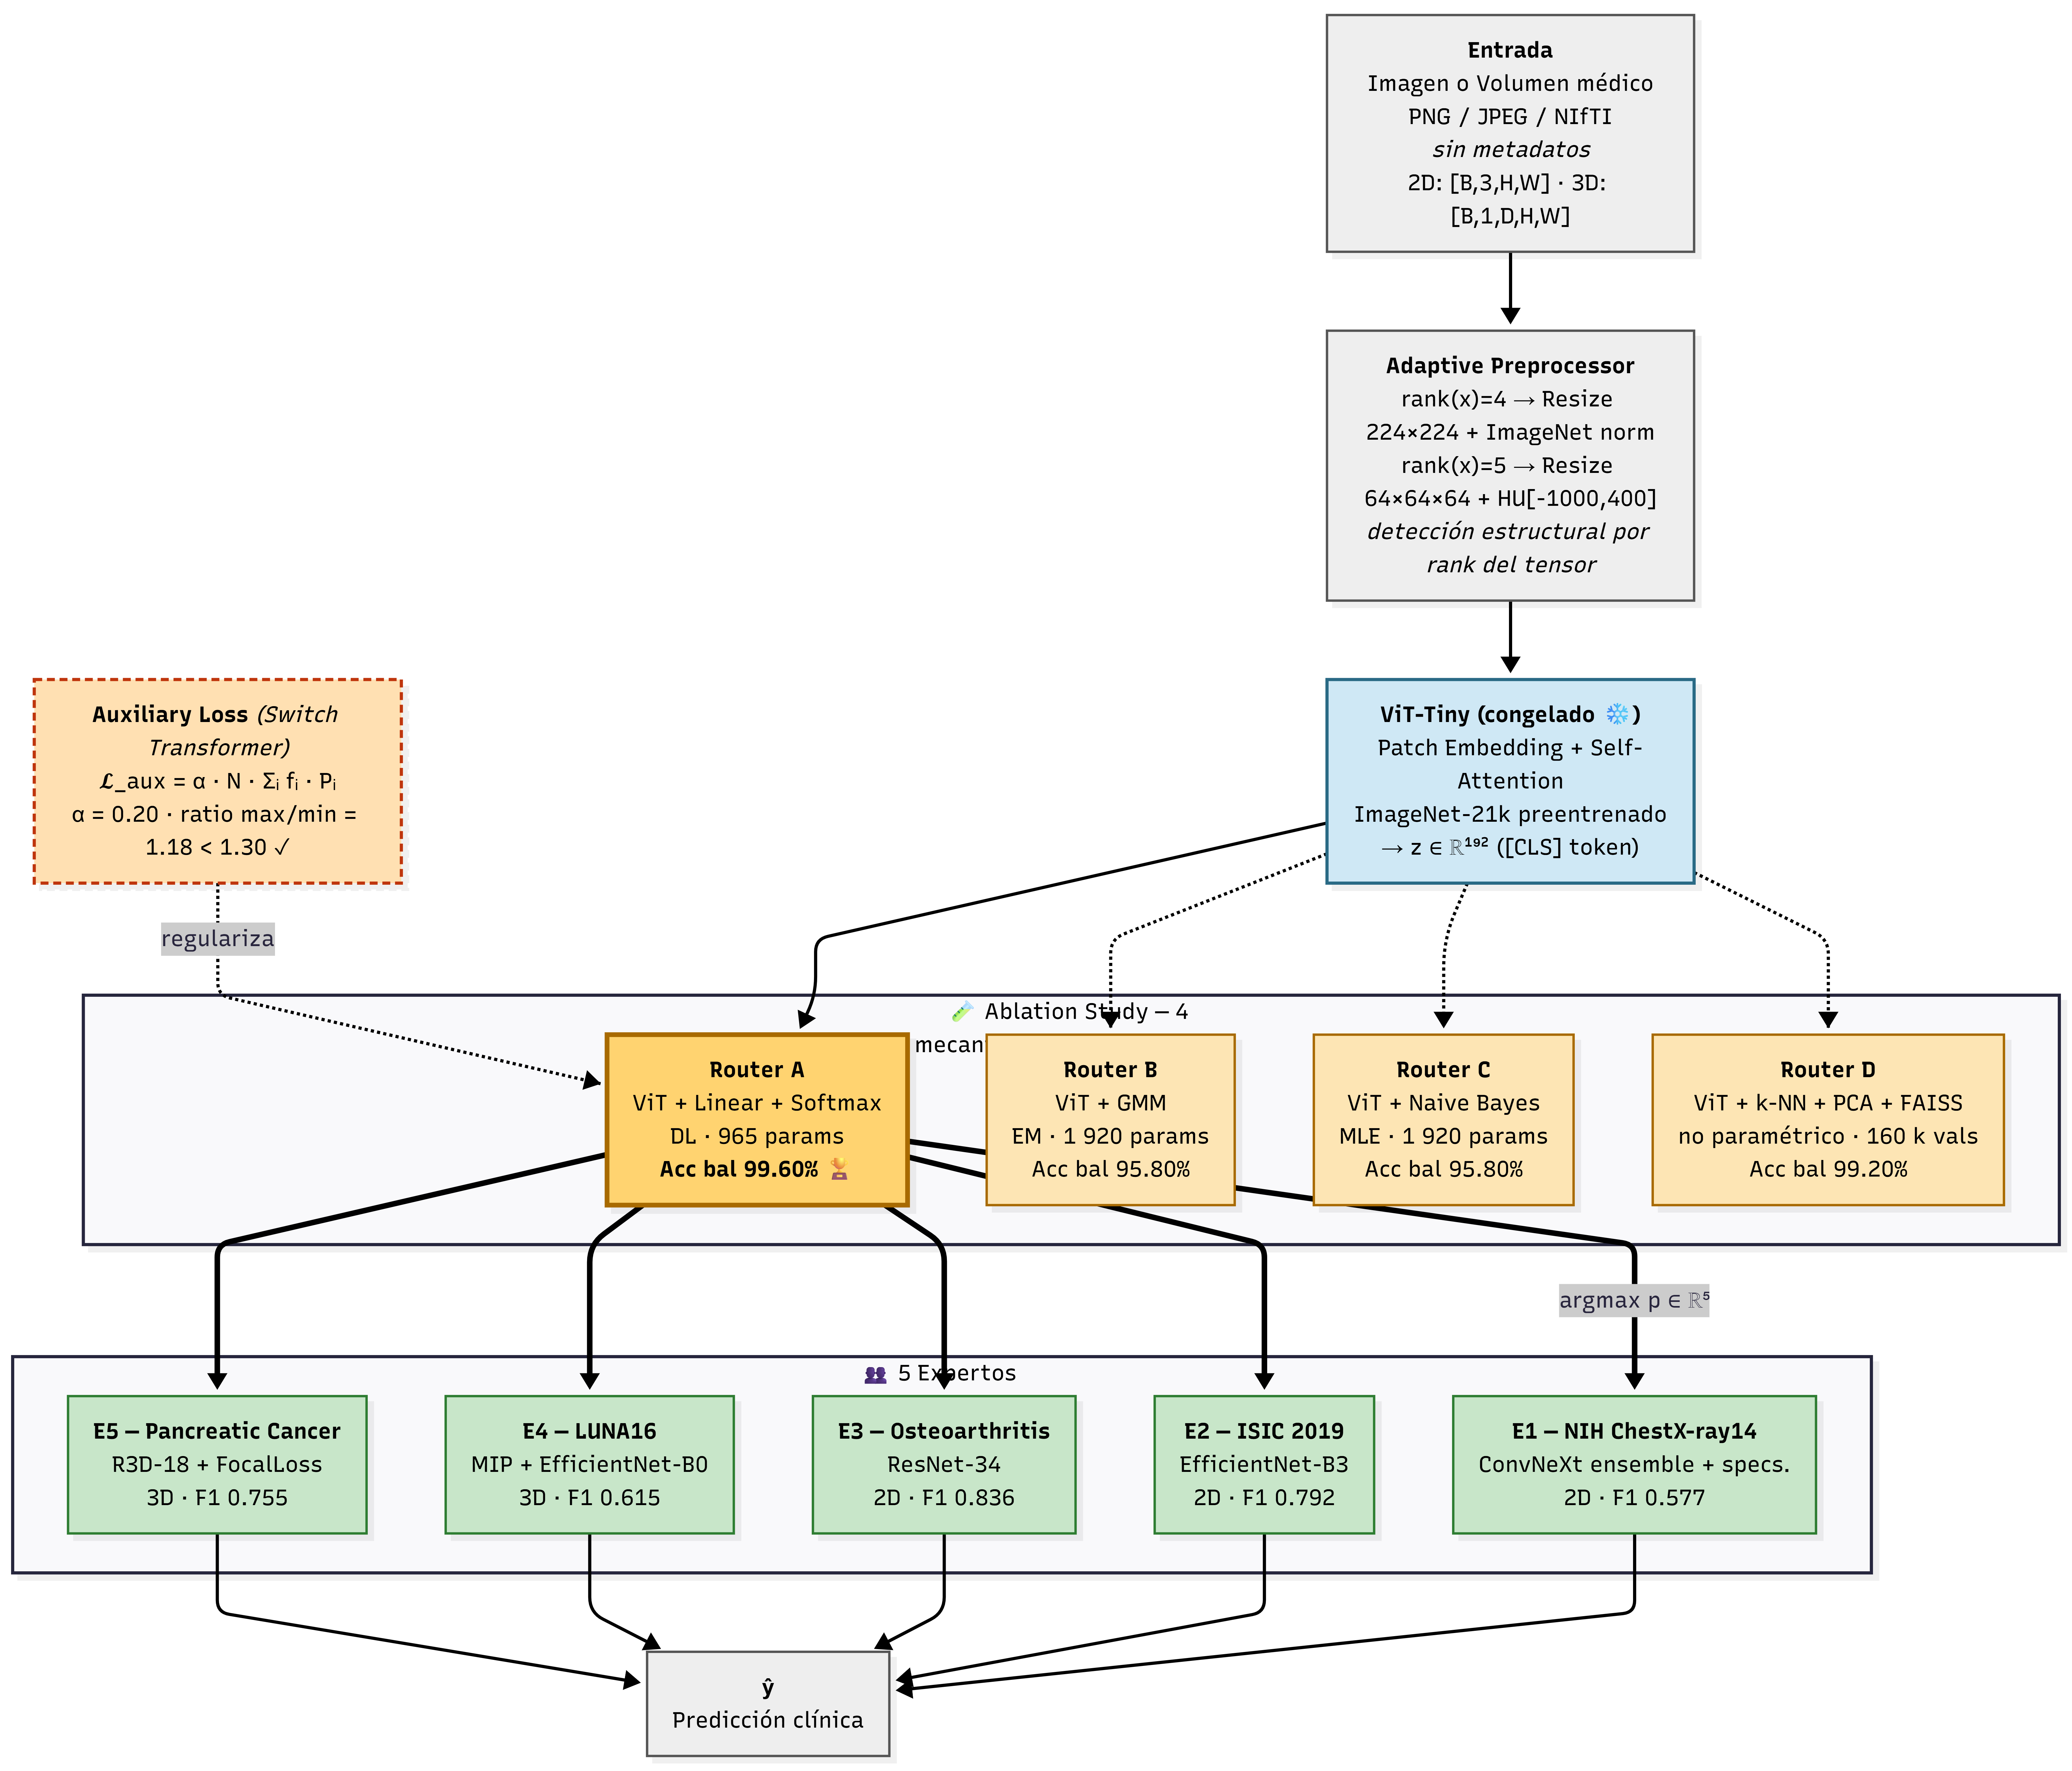
\includegraphics[width=\textwidth,height=0.80\textheight,keepaspectratio]{grafica_arquitectura_mermaid.png}
\end{frame}

\begin{frame}{5. Ablation Study -- los 4 mecanismos}
\small
\begin{tabularx}{\textwidth}{>{\bfseries}l Y Y}
\toprule
Router & Naturaleza & Ecuacion clave \\
\midrule
A -- ViT + Linear & DL (gradiente) & $g(z)=\mathrm{softmax}(Wz+b)$ \\
B -- GMM & Parametrico (EM) & $P(e_i\mid z) \propto \pi_i\,\mathcal{N}(z;\mu_i,\Sigma_i)$ \\
C -- Naive Bayes & Parametrico (MLE, analitico) & $\prod_j \mathcal{N}(z_j;\mu_{ij},\sigma^2_{ij})$ \\
D -- k-NN + PCA & No parametrico & $\arg\max_i \sum_{j\in\mathrm{kNN}} \mathbb{1}[e_j=i]$ \\
\bottomrule
\end{tabularx}

\vspace{0.25cm}
\begin{itemize}
  \item PCA 192$\to$32 para D (varianza explicada 84.5\%) para mitigar la maldicion de dimensionalidad.
  \item Embeddings extraidos una sola vez: $Z_{\mathrm{train}}\in\mathbb{R}^{121287\times192}$.
\end{itemize}
\end{frame}

\begin{frame}{6. Evaluacion justa -- subset balanceado}
\begin{block}{Problema}
El conjunto de validacion natural esta dominado por NIH (77\%). Un router ingenuo que siempre diga \texttt{NIH} obtendria \textasciitilde77\% de accuracy, lo que vuelve la metrica enganosa.
\end{block}

\begin{block}{Solucion metodologica}
\begin{itemize}
  \item Muestreo estratificado: 1 000 por clase en train (5 000 total) y 200 por clase en val balanceado.
  \item Se reportan dos metricas:
    \begin{itemize}
      \item \textbf{Acc. (bal)}: capacidad discriminativa pura.
      \item \textbf{Acc. (full)}: comportamiento operativo bajo la distribucion real.
    \end{itemize}
\end{itemize}
\end{block}

La brecha entre ambas es un \textbf{diagnostico}: mide cuanto depende el router de la prior empirica.
\end{frame}

\begin{frame}{7. Resultados del ablation study}
\small
\begin{tabularx}{\textwidth}{>{\bfseries}Y c c c c c}
\toprule
Router & Acc. bal & Acc. full & Latencia & Params & GPU \\
\midrule
A -- ViT + Linear & \textbf{99.60\%} & \textbf{98.27\%} & 0.000 ms & 965 & Si \\
D -- k-NN + PCA & 99.20\% & 97.11\% & 1.447 ms & 160 000 & No \\
B -- GMM & 95.80\% & 87.35\% & 0.004 ms & 1 920 & No \\
C -- Naive Bayes & 95.80\% & 87.34\% & 0.002 ms & 1 920 & No \\
\bottomrule
\end{tabularx}

\vspace{0.35cm}
\begin{itemize}
  \item \textbf{Los 4} superan la meta de 80\% en ambos regimenes.
  \item Router A gana; k-NN queda a menos de 1.2 pp en ambos regimenes.
  \item GMM y NB son practicamente indistinguibles entre si.
\end{itemize}
\end{frame}

\begin{frame}{8. Discusion -- \textquestiondown que nos dicen los numeros?}
\begin{itemize}
  \item \textbf{Hipotesis natural (ViT gana):} \cmark\ confirmada, pero \textbf{matizada}.
  \item Diferencia A vs.
    \begin{itemize}
      \item k-NN: \textbf{0.40 pp} (bal) / \textbf{1.16 pp} (full)
      \item Naive Bayes: \textbf{3.8 pp} (bal)
    \end{itemize}
\end{itemize}

\vspace{0.25cm}
\begin{block}{Leccion principal}
\centering
\large La \textbf{calidad del embedding} importa mas que la complejidad del routing.\\[0.15cm]
Un ViT bien preentrenado genera representaciones donde hasta \textbf{Naive Bayes} supera el 95\% balanceado.
\end{block}

\vspace{0.15cm}
\textbf{Implicacion practica:} en hardware restringido, \textbf{k-NN+PCA} o \textbf{Naive Bayes} son alternativas viables (sin GPU, 0.002 ms).
\end{frame}

\begin{frame}{9. Variante jerarquica 2D+3D}
\begin{block}{Diagnostico runtime}
Auditoria sobre 50 imagenes crudas: el Router A 5-clases cae a \textbf{58\%} end-to-end. NIH y OA colapsan al experto 3 por desbalance espacial residual ausente en embeddings pre-computados.
\end{block}

\begin{block}{Refinamiento}
El preprocesador \textbf{ya conoce} el rango del tensor $\Rightarrow$ split 2D/3D deterministico (error estructural 0\%). Dos cabezas lineales independientes sobre $z$:
\end{block}

\small
\begin{tabularx}{\textwidth}{>{\bfseries}l Y c c}
\toprule
Router & Clases & Train & Acc. bal \\
\midrule
Router 2D & NIH / ISIC / OA & 1 500/clase & \textbf{99.50\%} \\
Router 3D & LUNA / Pancreas & 160/clase & \textbf{100\%} \\
\midrule
 & \textbf{Fusion ponderada} & & \textbf{99.56\%} \\
\bottomrule
\end{tabularx}

\vspace{0.2cm}
Equivalente al Router A plano pero elimina confusiones inter-modalidad en runtime.
\end{frame}

\begin{frame}{10. Balance de carga -- Auxiliary Loss}
\[
\mathcal{L}_{\mathrm{aux}} = \alpha\, N \sum_{i=1}^{N} f_i\, P_i
\qquad (\alpha = 0.20)
\]

\begin{itemize}
  \item \textbf{Expert Collapse}: si el router siempre activa al mismo experto, se destruye la especializacion.
  \item \textbf{Rubrica:} $\max(f_i)/\min(f_i) < 1.30$; de lo contrario se pierde 40\% de la nota.
  \item \emph{Sweep} de $\alpha \in \{0.05, 0.10, 0.20\}$: $\alpha=0.20$ evita ratios transitorios mayores a 1.30.
\end{itemize}

\vspace{0.25cm}
\begin{block}{Resultado final}
\centering
\Large ratio = \textbf{1.18 $< 1.30$} \cmark
\end{block}
\end{frame}

\begin{frame}{11. Expertos heterogeneos -- resultados}
\small
\begin{tabularx}{\textwidth}{c Y Y c}
\toprule
Expert & Dataset & Arquitectura & F1 Macro \\
\midrule
1 & NIH ChestX-ray14 & \textbf{ConvNeXt ensemble + especialistas Mass/Nodule} & 0.577 \\
2 & ISIC 2019 & EfficientNet-B3 & 0.792 \\
3 & Osteoarthritis & ResNet-34 & \textbf{0.836} \\
4 & LUNA16 & MIP + EfficientNet-B0 & 0.615 \\
5 & Pancreatic & R3D-18 + FocalLoss & 0.755 \\
\bottomrule
\end{tabularx}

\vspace{0.25cm}
\begin{itemize}
  \item \textbf{Experto 1 (NIH):} de DenseNet-121 multi-label (F1 = 0.327) a ConvNeXt + 2 especialistas + umbral re-ajustado $\Rightarrow$ F1 = 0.577 (\textbf{+25 pp}).
  \item Meta 2D $>0.72$ \cmark\ (E2, E3). Meta 3D $>0.65$ \cmark\ (E5). E1 y E4 quedan por debajo por clases de baja prevalencia.
\end{itemize}
\end{frame}

\begin{frame}{12. Evaluacion end-to-end y OOD}
\small
\begin{tabularx}{\textwidth}{Y c c c c}
\toprule
Dominio & $N_{\mathrm{val}}$ & Route Acc. & F1 Expert & F1 E2E \\
\midrule
NIH & 16 818 & 0.9934 & 0.577 & 0.573 \\
ISIC & 3 799 & 0.9958 & 0.792 & 0.789 \\
Osteoarthritis & 953 & 0.9990 & 0.836 & 0.835 \\
LUNA16 MIP & 177 & 1.0000 & 0.615 & 0.615 \\
\midrule
 &  &  & \textbf{Macro} & \textbf{0.7030} \\
\bottomrule
\end{tabularx}

\vspace{0.25cm}
\begin{block}{Calibracion del router como detector OOD}
\begin{itemize}
  \item AUROC = 0.9845 sin entrenamiento adicional.
  \item $\tau = 0.95$: cubre 96.8\% con accuracy 0.9994 $\Rightarrow$ \emph{reject-option} gratis.
\end{itemize}
\end{block}
\end{frame}

\begin{frame}{13. Dashboard interactivo}
\begin{block}{Funcionalidades implementadas}
\begin{itemize}
  \item Carga de PNG / JPEG / NIfTI con deteccion automatica 2D/3D.
  \item Inferencia en tiempo real: etiqueta, confianza y latencia.
  \item \textbf{Attention heatmap} del router ViT (rollout Abnar \& Zuidema).
  \item Panel del experto activado + \emph{gating score}.
  \item Tabla del ablation study con los 4 routers y sus metricas reales.
  \item Barras de load balance ($f_i$ acumulado).
  \item Alerta OOD cuando la entropia del gating supera el umbral.
  \item Selector Router A / Router D (k-NN) para demo comparativa.
\end{itemize}
\end{block}
\end{frame}

\begin{frame}{14. Alcances y limitaciones}
\begin{columns}[T,totalwidth=\textwidth]
\column{0.5\textwidth}
\begin{block}{Alcances \cmark}
\begin{itemize}
  \item Preprocesador adaptativo sin metadatos para 5 modalidades.
  \item Los 4 routers superan 80\%; la pregunta cientifica queda respondida.
  \item Balance de carga dentro del umbral (ratio 1.18 $< 1.30$).
  \item Dashboard con heatmap, OOD y selector de routers.
\end{itemize}
\end{block}

\column{0.5\textwidth}
\begin{block}{Limitaciones \xmark}
\begin{itemize}
  \item Expertos 3D entrenados sobre subsets (LUNA 888 vol., Pancreas \textasciitilde558 vol.).
  \item El router de LUNA usa un \emph{proxy} MIP, no el volumen 3D real.
  \item NIH se entrena sobre 5 patologias, no 14; Mass y Nodule siguen afectando el F1 macro.
\end{itemize}
\end{block}
\end{columns}

\vspace{0.2cm}
\textbf{Con mas tiempo:} backbone 3D medico (MedicalNet), datasets completos y Top-K gating.
\end{frame}

\begin{frame}[plain]
\vspace{0.5cm}
{\color{uaoblue}\LARGE\bfseries 15. Conclusiones\par}
\vspace{0.4cm}
\begin{itemize}
  \item La pregunta cientifica queda respondida con datos: el ViT justifica su costo en precision, pero por un margen pequeno.
  \item \textbf{La calidad del embedding $>$ la complejidad del routing}: con ViT-Tiny preentrenado, hasta Naive Bayes supera el 95\% balanceado.
  \item Sistema MoE integrado: \textbf{99.60\%} routing acc. balanceada, \textbf{F1 macro E2E = 0.7030} y ratio de balance \textbf{1.18}.
  \item El valor principal del proyecto esta en el \textbf{diseno experimental honesto}, no en forzar que ViT gane por mucho.
\end{itemize}

\vfill
\centering
\Large\textbf{Gracias -- \textquestiondown preguntas?}
\end{frame}

\end{document}
